
\chapter{C++ Implementation}





\section{C++ Language Background I}





Member functions like those shown are represented by normal functions, 
with additional hidden parameter, \lstinline{pThis} representing \lstinline{this}. 
To call a member function of an object, \lstinline{a.f(x,y,z)} we push 
\textit{four} parameters. We push \lstinline{x}, \lstinline{y}, \lstinline{z}, 
as usual however, we \textit{also} push the the pointer to \lstinline{a}'s object space. 
This is what parameter \lstinline{pThis} will be bound to.

Given
%\lstinline{class S} \lstinline{\{} \lstinline{public} \lstinline{\{}
%\lstinline{void} \lstinline{f} \lstinline{(..)} \lstinline{\{} 
%\lstinline{..} \lstinline{\}} \lstinline{\}},

\highlightdef{To call member function \lstinline{f},
we have an \textit{hidden parameter} to \\
bind \lstinline{this} to the receiver object.}

We can have several objects of one class, but only one copy of the instructions exist.

\begin{figure}[h]
\begin{tikzpicture}[
  title/.style={},
  object/.style={rectangle split, rectangle split draw splits=false,
  draw, text width=2cm}
]

  \node[rectangle split, rectangle split horizontal, rectangle split parts=3, 
  draw, text width=1cm, anchor=center, text centered]
  (t){ 
  \lstinline{S_f} 
  \nodepart{two} 
  \lstinline{S_g} 
  \nodepart{three} 
  \lstinline{T_f}
  };

\end{tikzpicture}
\end{figure} 


Noticed how we combined the class name and the member function name together 
to create unique identifiers for instance method bodies. 
If two classes have the same member function name, the identifier 
$\langle \text{classid} \rangle \_ \langle \text{memfuncid} \rangle$
will uniquely identiy the instance method. 

This idea of creating unique identifers by combining names is 
called \textit{name mangling}. It's a common technique used by compilers. 

\highlightdef{\textbf{Name mangling} allows distinction between
member functions of different classes}

We didn't have to choose 
$\langle \text{classid} \rangle \_ \langle \text{memfuncid} \rangle$
for our name mangling. Instead, we could've used 
$\langle \text{memfuncid} \rangle \_ \langle \text{classid} \rangle$.
Name mangling is also used to distinguish overloaded member functions 
for a given classes. The parameter names and types would be used in the 
name mangling process.

\frmrule



The \textit{behaviour} of \lstinline{a} is statically-bound to the member functions in the $A$ table. 
The assignment \lstinline{a1 = b1;} changed only the \textit{state} of $a1$ (values of field variables), 
but the \textit{behaviour} (member functions associated) is unchanged. However this is only the case 
for object assignment. Pointers with pointer assignment behave differently. 

\frmrule

\begin{example}
The example below highlights the difference between static binding and dynamic binding.

\begin{figure}[h]
\begin{tikzpicture}
  \node [fill=black!5, inner sep=4pt] (class) { 
  
\begin{lstlisting}
class A { public:
 virtual int f() { return 10; };
         int g() { return 15; };
};
class B : public A  { public:
 virtual int f() { return 20; };
         int g() { return 25; };
};
\end{lstlisting} 
  };

  \node [fill=black!5, inner sep=4pt, right=0.05cm of class] (static) { 
\begin{lstlisting}
void main()
{
 A a1; B b1;

 a1.f(); //10
 a1.g(); //15

 b1.f(); //20
 b1.g(); //25

 a1 = b1;
 a1.f(); //10
 a1.g(); //15
};
\end{lstlisting} 
  };

  \node [fill=black!5, inner sep=4pt, right=0.05cm of static] { 
\begin{lstlisting}
void main() 
{
 A* ap1; B* bp1;

 ap1->f(); //10
 ap1->g(); //15

 bp1->f(); //20
 bp1->g(); //25

 ap1 = bp1;
 ap1->f(); //20
 ap1->g(); //15
};
\end{lstlisting} 
  };

\end{tikzpicture}
\end{figure} 



\end{example}


C++ has two binding modes, static-binding and dynamic binding. 
Static binding is used for object instances and dynamic binding is 
used for object pointers.
\highlightdef {
  \textbf{Static binding}: always used for object values \\
  \textbf{Dynamic binding}: only possbile for object pointers 
}

Virtual functions may be bound dynamically. When a 
virtual function is called for pointer, then the function 
is bound according to the class of the object pointed at 
by pointer, and not according to the type of pointer. 

In other OO languages, e.g. Smalltalk, Java, there is \textit{only dynamic binding}. 
Which mode is more important for OO? Why are there two modes of 
binding in C++? How many modes of binding for C\#? 

\frmrule


\begin{example}
This example shows how dynamic binding is continued throughout nested calls


\begin{figure}[h]
\begin{tikzpicture}
  \node [fill=black!5, inner sep=4pt] (class) { 
  
\begin{lstlisting}
class A { public:
 virtual int f() { return 10;  };
         int g() { return 15;  };
};
class B : public A { public:
 virtual int f() { return g(); };
         int g() { return 20;  };
};
class C : public B { public:
         int g() { return 25;  };
};
\end{lstlisting} 
  };

  \node [fill=black!5, inner sep=4pt, right=0.05cm of class] (static) { 
\begin{lstlisting}
void main()
{
 A a1; 
 C c1;

 a1.f(); //
 a1.g(); //

 c1.f(); //
 c1.g(); //
};
\end{lstlisting} 
  };

  \node [fill=black!5, inner sep=4pt, right=0.05cm of static] { 
\begin{lstlisting}
void main() 
{
 A* ap1=new A(); 
 C* cp1=new C(); 

 ap1->f(); //
 ap1->g(); //

 cp1->f(); //
 cp1->g(); //
};
\end{lstlisting} 
  };

\end{tikzpicture}
\end{figure} 

\end{example}

\frmrule

\begin{example}
This example shows dynamic binding related errors.


\begin{figure}[h]
\begin{tikzpicture}
  \node [fill=black!5, inner sep=4pt] (class) { 
  
\begin{lstlisting}
class A { public:
 virtual int f() { return 10;  };
};
class B : public A { public:
 int i;
 virtual int f() { return g()+i; };
         int g() { return 20;  };
};
\end{lstlisting} 
  };

  \node [fill=black!5, inner sep=4pt, right=0.05cm of class] (static) { 
\begin{lstlisting}
void main()
{
 A a1; 
 C c1;

 a1.f(); //
 a1.g(); //

 c1.f(); //
 c1.g(); //
};
\end{lstlisting} 
  };

  \node [fill=black!5, inner sep=4pt, right=0.05cm of static] { 
\begin{lstlisting}
void main() 
{
 A* ap1=new A(); 
 B* bp1=new C(); 
 bp1->i = 100;

 ap1->f(); //10
 bp1->f(); //120
 bp1->g(); //20

 ap1= bp1;
 ap1->f(); //10
 ap1->g(); //!
 ap1->g(); //!
};
\end{lstlisting} 
  };

\end{tikzpicture}
\end{figure} 

\end{example}




\section{C++ Language Background II}





\begin{lstlisting}
class S {
	void u() {}; void v() {}; void w() {};
}
class T : public S {
	void u() {};
}
\end{lstlisting}


\begin{figure}[h]
\begin{tikzpicture}[
  title/.style={},
  object/.style={rectangle split, rectangle split draw splits=false,
  draw, text width=2cm}
]

  \node[rectangle split, rectangle split horizontal, rectangle split parts=4, 
  draw, text width=1cm, anchor=center, text centered]
  (t){ 
  \lstinline{S_u} 
  \nodepart{two} 
  \lstinline{S_v} 
  \nodepart{three} 
  \lstinline{S_w}
  \nodepart{four} 
  \lstinline{T_u}
  };

\end{tikzpicture}
\end{figure} 


Below shows how fields are inherited.

\begin{lstlisting}
class S {
	int a; int b; int c;
}
class T : public S {
	int x;
}
\end{lstlisting}


\begin{figure}[h]
\begin{tikzpicture}[
  title/.style={},
  object/.style={rectangle split, rectangle split draw splits=false,
  draw, text width=2cm}
]

  \node[rectangle split, rectangle split horizontal, rectangle split parts=3, 
  draw, text width=1cm, text centered]
  (t1){ 
  \lstinline{s1_a} 
  \nodepart{two} 
  \lstinline{s1_b} 
  \nodepart{three} 
  \lstinline{s1_c}
  };

  \node[rectangle split, rectangle split horizontal, rectangle split parts=4, 
  draw, text width=1cm, text centered, below=1cm of t1]
  (t2){ 
  \lstinline{t1_a} 
  \nodepart{two} 
  \lstinline{t1_b} 
  \nodepart{three} 
  \lstinline{t1_c}
  \nodepart{four} 
  \lstinline{t1_x}
  };


\end{tikzpicture}
\end{figure} 





The table used for accessing virtual member functions is called 
the \textit{virtual table}, and a pointer to it is represented by a 
field vtab. 

\highlightdef{Only virtual member functions are put in virtual tables.}

Normal (non-virtual) member functions will not be found in the method table 
for a class. 

We'll use a double letter convention 
\lstinline{ff}, \lstinline{gg}, \lstinline{hh} ... for virtual member functions.

\highlightdef{If $C < D$, then $\text{vtab}_C$ is a prefix of $\text{vtab}_D$}




\section{High Level Target Language I}

We can get a high level view of the changes a compiler makes.
We can abstract compilation features we are not interested in
and concentrating the featues we are interested in. 
For us, we are interested in reasoning about high level features. 
We are not interested in details such as 
memory alignment, types, sizes, machine code instructions.
In fact, we abstract away enough so our view will be independent of 
any machine's instruction set.

\begin{itemize}   
\renewcommand{\labelitemi}{$\Box$}
\item \textbf{Identifiers} The set $Ident$ is a set of identifiers $x$. 
\item \textbf{Memory} A given memory $m$ is a map $m : Int \rightarrow Int \cup Ident$ to the set. 
We assume a word addressed machine. $m(x)$ addresses word number $x$. 
We assume that identifier addresses take up \textit{one word}. 
There is a \textit{position function} $\pi : Ident \rightarrow int$ gives a memory for each identifier.
\end{itemize} 

The syntax of the C++ HLTL is shown below.

$$Loc ::= IntConst \;|\; \alpha(Ident) \;|\; \star Loc \;|\; Loc + Loc $$


Now we describe the operation semantics for $Loc$.
We define a location evaluation $\leadsto_L$. 

\highlightdef{\textbf{Location Evaluation}: 
$\leadsto_L : Int \times (Ident \rightarrow Int) 
\times (Int \rightarrow Int \cup Ident) \rightarrow Int$ }


\begin{prooftree}
\def\defaultHypSeparation{\hskip .01in}
\AxiomC{}
\LeftLabel{\textsc{const}}
\UnaryInfC{$(i, \pi, m) \leadsto_L i$}
\end{prooftree}

This first axiom states that a constant integer representing 
the address of word in memory evaluates to that very constant integer. 

\begin{prooftree}
\def\defaultHypSeparation{\hskip .01in}
\AxiomC{}
\LeftLabel{\textsc{pos}}
\UnaryInfC{$(\alpha(x), \pi, m) \leadsto_L \pi(i)$}
\end{prooftree}

The next axiom is for the identifier \textit{position operator} $\alpha$. The rule says that 
the deferencing operator gives the location of an identifer, 
which is given by the \textit{position function} $\pi$. 
Note that the difference between $\alpha$ and $\pi$ is that 
$\alpha$ is part of the syntax of the high level target language - 
whereas $\pi$ is not. We use $\pi$ to, describe the operational semantics
of $\alpha$, and to describe other semantics. 

\begin{prooftree}
\def\defaultHypSeparation{\hskip .01in}
\AxiomC{$(loc, \pi, m) \leadsto_L i$}
\LeftLabel{\textsc{deref}}
\UnaryInfC{$(\star loc, \pi, m) \leadsto_L m(i)$}
\end{prooftree}

The next rule is for the deferencing operator $\star$. Given any location 
$loc$, we use $\star$ to see the \textit{contents} of the memory address 
that $loc$ refers to. If $loc$ location-evaluated to $i$, then the location 
$loc$ refers to is $i$ and so the memory contents are given by $m(i)$.  
So overall, $\star loc$ location-evaluates to $m(i)$. 

\begin{prooftree}
\def\defaultHypSeparation{\hskip .01in}
\AxiomC{$(loc, \pi, m) \leadsto_L i$}
\AxiomC{$(loc', \pi, m) \leadsto_L i'$}
\LeftLabel{\textsc{add}}
\BinaryInfC{$(loc + loc', \pi, m) \leadsto_L i + i'$}
\end{prooftree}

The next rule allows us to add two addresses together. 
We define the semantics for $Loc + Loc$. Suppose we 
have two locations $loc,loc' \in Loc$.  
Intuitively, if location $loc$ evaluates to integer $i$ and 
another location $loc'$ evaluates to integer $i'$ then 
$loc + loc'$ evaluates to integer $i + i'$. 

\frmrule

\begin{example}



\end{example}

\frmrule  

We now add instructions to HLTL. 
Instructions allow us to modify the contents of memory. Below shows the syntax 
for instructions $Instr$ and method bodies $MethBody$.

$$Instr ::= Instr;Instr \;|\; Loc := Loc \;|\; Ident(Loc^{*}) \;|\; Loc(Loc^{*}) $$
$$MethBody ::= Ident^{*} \{ Instr^{*} \}$$

Now we describe the operation semantics for instructions by
defining an instruction evaluation $\leadsto_I$. 

\highlightdef{\textbf{Instruction Evaluation}: 
$\leadsto_I : Instr \times (Ident \rightarrow Int) \times (Int \rightarrow Int \cup Ident)
\rightarrow (Int \rightarrow Int \cup Ident)$ }


\begin{prooftree}
\def\defaultHypSeparation{\hskip .01in}
\AxiomC{$(loc := loc', \pi, m) \leadsto_I i$}
\AxiomC{$(loc := loc', \pi, m) \leadsto_I i'$}
\LeftLabel{\textsc{assign}}
\BinaryInfC{$(loc := loc', \pi, m) \leadsto_I m[i \mapsto i']$}
\end{prooftree}

This rule updates the memory to reflect an assignment. 
The location indicated by $loc$ is updated to the location indiciated 
by $loc'$. If $loc'$ location-evaluates to $i'$ then this is what should 
be in whatever location $loc'$ location-evaluates to, $i$. 
Hence the instruction updates the memory function $m$ to $m[i \mapsto i']$ 
where all mappings are unchanged except that now $i$ maps to $i'$. 

\begin{prooftree}
\def\defaultHypSeparation{\hskip .01in}
\AxiomC{$(instrs, \pi, m) \leadsto_I m'$}
\AxiomC{$(instr, \pi, m') \leadsto_I m''$}
\LeftLabel{\textsc{seq}}
\BinaryInfC{$(instrs;instr, \pi, m) \leadsto_I m''$}
\end{prooftree}

The next rule is for creating sequences of instructions. 
The rule tells us that the evaluation of $instrs;instr$ 
requires that we instruction-evaluate $instrs$, then take the 
memory contents of that evaluation and 
use them to instruction-evaluate $instr$ to give the final memory 
contents.



\begin{prooftree}
\def\defaultHypSeparation{\hskip .01in}
\AxiomC{
$
\begin{matrix}
&
\kappa(id) = par_1 \cdots par_n \{ instrs \}
&
\\
\begin{matrix}
(loc_1, \pi, m) \leadsto_L i_1  \\
(loc_2, \pi, m) \leadsto_L i_2  \\
\cdots \\
(loc_n, \pi, m) \leadsto_L i_n \\
(instrs, \pi', m') \leadsto_I m'' \\
\end{matrix}
&
\pi' =
\begin{matrix}
par_1 \mapsto i_1'  \\
par_2 \mapsto i_2'  \\
\cdots \\
par_n \mapsto i_n'
\end{matrix}
&
m' = m\left[
\begin{matrix}
i_1' \mapsto i_1  \\
i_2' \mapsto i_2  \\
\cdots \\
i_n' \mapsto i_n
\end{matrix}\right]
\end{matrix}
$
}
\LeftLabel{\textsc{func}}
\UnaryInfC{$(id(loc_1, \cdots, loc_n), \pi, m) \leadsto_I m''$}
\end{prooftree}


When we call a method, the idea is to create a new scope. 
We need to find a way to binds the parameters identifiers $par_1 \cdots, par_n$
to our argument identifiers $loc_1 \cdots, loc_n$.  
Suppose that the arguments $loc_1 \cdots, loc_n$ location-evaluate to $i_1, \cdots i_n$ , 
then it is these memory locations that hold the argument values. 
In essence, $i_1, \cdots i_n$ are integer constants that are 
\textit{references} to the argument values. 
Performing $\star i_k$ gives the $k$th argument's value. 



\begin{tikzpicture}
  %
  \tikzstyle{m} = [draw=black!50, minimum width=1.5cm, minimum height=0.5cm, inner sep = 0.2pt, font=\small]
  \tikzstyle{m2} = [m, fill=black!5, draw=black!50]
  \matrix[row sep=-0.01cm, column sep=-0.01cm] (memory) 
  {
    \node[m]{}; & \node[m]{}; \\
    \node[m]{}; & \node[m]{}; \\
    \node[m]{}; & \node[m]{}; \\
    \node[m]{}; & \node[m]{}; \\
    \node[m2](i1){$i_1'$}; & \node[m2]{$i_1$}; \\
    \node[m2](i2){$i_2'$}; & \node[m2]{$i_2$}; \\
    \node[m2](ietc){$\cdots$}; & \node[m2]{$\cdots$}; \\
    \node[m2](in){$i_n'$}; & \node[m2]{$i_n$}; \\
  };
  \node[left=1.4cm of i1](par1){$par_1$}; 
  \node[left=1.4cm of i2](par2){$par_2$}; 
  \node[left=1.4cm of ietc](paretc){$\cdots$}; 
  \node[left=1.4cm of in](parn){$par_n$}; 
  \draw[|->,>=stealth',shorten >=3pt] (par1) -- (i1);
  \draw[|->,>=stealth',shorten >=3pt] (par2) -- (i2);
  \draw[|->,>=stealth',shorten >=3pt] (paretc) -- (ietc);
  \draw[|->,>=stealth',shorten >=3pt] (parn) -- (in);
  \node at ($(par1)+(1.0cm,0.5cm)$) {$\pi'$};
  \draw[decorate,decoration={brace},thick]
      ($(memory.north west)+(0.1cm,0.1cm)$) to node[midway,above,yshift=0.1cm] {$m'$}
      ($(memory.north east)+(-0.1cm,0.1cm)$);
\end{tikzpicture}



% Add Prooftree


Now we need to decide whether to \textit{pass by value} or we \textit{pass by reference}.
We have decided to write the operational semenatics such that every parameter for 
every method call uses \textit{pass by value}. We need to work out how to 
create references to our parameter values. 

Notice that if we did \textit{pass by reference}, then our parameters would location-evaluate to 
$i_1, \cdots i_n$, just as how location-evaluating the arguments themselves gives 
$i_1, \cdots i_n$. Our parameters would simply be aliases.
However we are adopting \textit{pass by value}. We don't want our 
parameters to evaluate directly to the memory addresses of the values. 
We need to add a level of indirection.
Instead, our parameters should location-evaluate to some new address $i_1', \cdots i_n'$ whose 
memory contents contain the direct memory addresses $i_1, \cdots i_n$ to the argument values. 

So to add this level of indirection, we add to memory $m$ new mappings, 
$m' = m[i_1' \mapsto i_1, i_2' \mapsto i_2, \cdots, i_n' \mapsto i_n]$, 
to create new addresses $i_1', \cdots i_n'$ whose 
memory contents contain the reference $i_1, \cdots i_n$ to the argument values. 
Now we just need to direct our parameters to $i_1', \cdots, i_n'$.

We create a new scope by creating a new $\pi'$ with 
just the mappings $par_1 \mapsto i_1'$, $par_2 \mapsto i_2'$, ..., $par_n \mapsto i_n'$
This allows our parameters to location-evaluate to the new address $i_1', \cdots, i_n'$. 


\begin{prooftree}
\def\defaultHypSeparation{\hskip .01in}
\AxiomC{
$
\begin{matrix}
(loc, \pi, m) \leadsto_L i \\
m(i) = id \\
(id(loc_1, \cdots, loc_n), \pi, m) \leadsto_I m'
\end{matrix}
$
}
\LeftLabel{\textsc{funcpoint}}
\UnaryInfC{$(loc(loc_1, \cdots, loc_n), \pi, m) \leadsto_I m'$}
\end{prooftree}


The next rule allows us to have \textit{function pointers}.
The previous rule only allows us to call functions using 
identifiers that are defined in $\kappa$. 
Rather than having just function calls via \textit{identifiers}, 
we could also have function calls via \textit{locations}.

If the memory contents given by some location $loc$ has a identifier $id$
and we know that a function call with that identifier is valid (it 
instruction evaluates to some memory) - 
then performing the function call \textit{using the location} 
makes sense. 

In essence, $loc$ acts as a function pointer. We are adding a level of 
indirection for calling functions. We can roughly think of 
$loc$ are pointing to a function $id$ that's defined in $\kappa$.
We can change the function that $loc$ points to by changing $m(i)$
from $id$ to some new $id'$ that's also has a mapping defined in $\kappa$. 


\frmrule

\begin{example}
Assume that $\pi(x) = 300, \pi(y) = 400$ for identifiers $x,y \in Ident$. \\
For the initial memory contents shown below, show the resulting memory 
after the execution of the following instructions.

$$\alpha(x) + 1 := \alpha(y); \;\;\;
\alpha(x)+2 := \star(\alpha(x)+1); \;\;\;
\alpha(x+3) := \star(\alpha(x))+1;$$

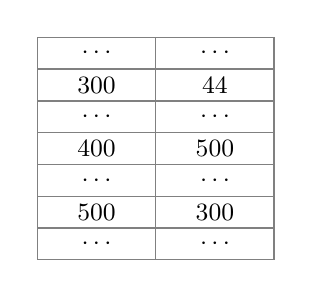
\begin{tikzpicture}
  %
  \tikzstyle{m} = [draw=black!50, minimum width=1.5cm, minimum height=0.4cm, inner sep=0.1pt, font=\small]
  \matrix[row sep=-0.01cm, column sep=-0.01cm] (memory) 
  {
    \node[m]{$\cdots$}; & \node[m]{$\cdots$}; \\
    \node[m]{300}; & \node[m]{44}; \\
    \node[m]{$\cdots$}; & \node[m]{$\cdots$}; \\
    \node[m]{400}; & \node[m]{500}; \\
    \node[m]{$\cdots$}; & \node[m]{$\cdots$}; \\
    \node[m]{500}; & \node[m]{300}; \\
    \node[m]{$\cdots$}; & \node[m]{$\cdots$}; \\
  };
\end{tikzpicture}
\end{example}

\frmrule

\begin{example}
Assume that $\pi(x) = 300, \pi(y) = 400$ for identifiers $x,y \in Ident$. \\
For the initial memory contents shown below, show the resulting memory 
after the execution of the following instructions.

$$
\star(\star(\alpha(y))) := 10; \;\;\;
\star(\alpha(x)) := 100; \;\;\;
\alpha(y) := 1000;
$$

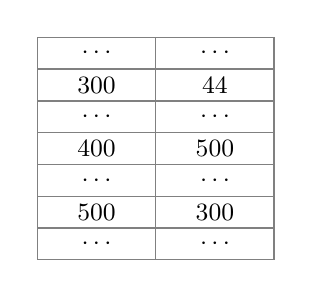
\begin{tikzpicture}
  %
  \tikzstyle{m} = [draw=black!50, minimum width=1.5cm, minimum height=0.4cm, inner sep=0.1pt, font=\small]
  \matrix[row sep=-0.01cm, column sep=-0.01cm] (memory) 
  {
    \node[m]{$\cdots$}; & \node[m]{$\cdots$}; \\
    \node[m]{300}; & \node[m]{44}; \\
    \node[m]{$\cdots$}; & \node[m]{$\cdots$}; \\
    \node[m]{400}; & \node[m]{500}; \\
    \node[m]{$\cdots$}; & \node[m]{$\cdots$}; \\
    \node[m]{500}; & \node[m]{300}; \\
    \node[m]{$\cdots$}; & \node[m]{$\cdots$}; \\
  };
\end{tikzpicture}
\end{example}

\frmrule

\begin{example}
Assume $\kappa(f) = x,y \{ \star \alpha(y) := \star \star \alpha(x) \}$. \\
For the initial memory contents shown below, show the resulting memory \\
\textbf{(a)} On entry to function $f$ for some $m, \pi'$ \\
\textbf{(b)} Just before leaving function $f$ for $m', \pi'$ \\
\textbf{(c)} After execution of the function $f$ for $m'', \pi$ \\

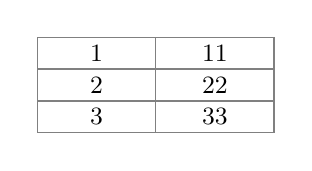
\begin{tikzpicture}
  %
  \tikzstyle{m} = [draw=black!50, minimum width=1.5cm, minimum height=0.4cm, inner sep=0.1pt, font=\small]
  \matrix[row sep=-0.01cm, column sep=-0.01cm] (memory) 
  {
    \node[m]{1}; & \node[m]{11}; \\
    \node[m]{2}; & \node[m]{22}; \\
    \node[m]{3}; & \node[m]{33}; \\
  };
\end{tikzpicture}
\end{example}

\frmrule



\section{High Level Target Language II}

We now extend the HLTL to suppose classes and objects. 

\begin{itemize}   
\renewcommand{\labelitemi}{$\Box$}
\item \textbf{Object Layout} Lay out all fields of a class next to each 
other in memory. For each field we associated some offset $k$ where $k \geqslant 0$. 
The compiler remembers which field has what offset.  
In order to address an object, \textsf{a}, we always take the first cell, $\alpha(\textsf{a})$.
\item \textbf{Invariant for Layout}  The layout of objects of any class is 
a prefix of the layout of objects of any subclass. 
The result of this is that if \textsf{f} has offset $k$ for $\textsf{a}:\textsf{A}$, 
then \textsf{f} will also have offset $k$ for any $\textsf{a}':\textsf{A}'$ where $\textsf{A}' <: \textsf{A}$.
\item \textbf{Data Access} Offsets of data members are known at compile time. 
Thus data member access can be implemented through statically known offsets. 
\lstinline{a.f} in C++ has a location evaluation equivalent to $\star(\alpha(\textsf{a})) + k$ for some known offset $k$. 
\item \textbf{Pointer Data Access} 
A pointer \textsf{ap} that points to objects of class \textsf{A} 
can point to any subclass $\textsf{A}' <: \textsf{A}$. 
We can perform data member access using pointers.
\lstinline{a->f} in C++ has a location evaluation equivalent to $\alpha(\textsf{ap}) + k$ for 
some known offset $k$ taken from layouts for class \textsf{A}.
By our invariant for layout, 
if \textsf{f} has offset $k$ for $\textsf{a}:\textsf{A}$, 
then it must have offset $k$ for any $\textsf{a}':\textsf{A}'$ where $\textsf{A}' <: \textsf{A}$.
Hence $\star(\alpha(\textsf{ap})) + k$ will always access field \textsf{f}, regardless of 
what subclass \textsf{a} points to.
\item \textbf{Object Assignment} 
Assignment of objects corresponds to copying their fields. 
For the assignment \lstinline{a=x}.
if \textsf{a.f} is a field in \textsf{a} with offset $j$, 
then $\alpha(\textsf{x}) + j := \star(\alpha(\textsf{f})) + j$. 
That is, the contents of the field are updated to the 
location evaluation equivalent of doing a C++ data access.
Notice that $\textsf{x}:\textsf{\textsf{X}}' <: \textsf{A}$, then not all 
of it's fields will be updated. Only the fields that 
are in prefix. 
\item \textbf{Pointer Assignment} 
The assignment of pointers corresponds to 
copying of addresses. The object fields are unchanged. 
The assignment \lstinline{ap=bp} is represented as:
then $\alpha(\textsf{ap}) := \star \alpha(\textsf{bp})$. 
That is, the contents at address $\pi(\textsf{ap})$ are updated 
to the contents of $\pi(\textsf{bp})$. In other words
$m' = m[\pi(\textsf{ap}) \mapsto m(\pi(\textsf{bp}))]$.

\end{itemize} 

\frmrule

\begin{example}


\end{example}

\frmrule

\begin{tikzpicture}
  \node [fill=black!5, inner sep=4pt] (class) { 
  
\begin{lstlisting}
class A { 
 public:
  int fa1, fa2;
};
class B : public A { 
 public:
  int fb1;
};
\end{lstlisting} 
  };

  \node [fill=black!5, inner sep=4pt, right=0.1cm of class] { 
\begin{lstlisting}
void main()
{
 A a1; B b1;
 a.fa1 = 3; a.fa2 = 5;
 b.fa1 = 4; a.fa2 = 6; a.fb1 = 8;

 A *ap1 = new B();
 ap->fa1 = 5; ap->fa2 = 7;
 A *bp1 = new B();
 bp->fa1 = 1; bp->fa2 = 4; bp->fb1 = 9;
};
\end{lstlisting} 
  };

\end{tikzpicture}



\begin{tikzpicture}
  %
  \tikzstyle{m} = [draw=black!50, minimum width=1.5cm, minimum height=0.4cm, inner sep=0.1pt, font=\small]
  \tikzstyle{m2} = [m, minimum width=2.2cm]
  \tikzstyle{b} = [fill=black!10]

  \matrix[row sep=-0.01cm, column sep=-0.01cm] (mema) 
  {
    \node[m]{$\cdots$}; & \node[m]{$\cdots$}; \\
    \node[m,b](fa1){$\pi(\textsf{a1})$}; & \node[m,b]{3}; \\
    \node[m,b](fa2){$\pi(\textsf{a1})$+1}; & \node[m,b]{5}; \\
    \node[m]{$\cdots$}; & \node[m]{$\cdots$}; \\
  };
  \matrix[row sep=-0.01cm, column sep=-0.01cm, above right=0.0cm and 0.1cm of mema.north east, anchor=north west] (memb) 
  {
    \node[m]{$\cdots$}; & \node[m]{$\cdots$}; \\
    \node[m,b]{$\pi(\textsf{b1})$}; & \node[m,b](fa1end){4}; \\
    \node[m,b]{$\pi(\textsf{b1})+1$}; & \node[m,b](fa2end){6}; \\
    \node[m,b](fb1){$\pi(\textsf{b1})+2$}; & \node[m,b](fb1end){8}; \\
    \node[m]{$\cdots$}; & \node[m]{$\cdots$}; \\
  };

  \matrix[row sep=-0.01cm, column sep=-0.01cm, below right=0.6cm and 0.0cm of mema.south west, anchor=north west] (memap) 
  {
    \node[m2]{$\cdots$}; & \node[m2]{$\cdots$}; \\
    \node[m2]{$\pi(\textsf{ap1})$}; & \node[m2]{$m(\pi(\textsf{ap1}))$}; \\
    \node[m2]{$\cdots$}; & \node[m2]{$\cdots$}; \\
    \node[m2,b](fa1'){$m(\pi(\textsf{ap1}))$}; & \node[m2,b]{5}; \\
    \node[m2,b](fa2'){$m(\pi(\textsf{ap1}))+1$}; & \node[m2,b]{7}; \\
    \node[m2]{$\cdots$}; & \node[m2]{$\cdots$}; \\
  };

  \matrix[row sep=-0.01cm, column sep=-0.01cm, above right=0.0cm and 0.1cm of memap.north east, anchor=north west] 
  {
    \node[m2]{$\cdots$}; & \node[m2]{$\cdots$}; \\
    \node[m2]{$\pi(\textsf{bp1})$}; & \node[m2]{$m(\pi(\textsf{bp1}))$}; \\
    \node[m2]{$\cdots$}; & \node[m2]{$\cdots$}; \\
    \node[m2,b]{$m(\pi(\textsf{bp1}))$}; & \node[m2,b](fa1end'){1}; \\
    \node[m2,b]{$m(\pi(\textsf{bp1}))+1$}; & \node[m2,b](fa2end'){4}; \\
    \node[m2,b](fb1'){$m(\pi(\textsf{bp1}))+2$}; & \node[m2,b](fb1end'){9}; \\
    \node[m2]{$\cdots$}; & \node[m2]{$\cdots$}; \\
  };
  \begin{pgfonlayer}{background} 
      \node (l1) at ($(fa1end.east)+(1.2cm,0.0cm)$) {\textsf{fa1}}; \draw[thick] (fa1) -- (l1); 
      \node (l2) at ($(fa2end.east)+(1.2cm,0.0cm)$) {\textsf{fa2}}; \draw[thick] (fa2) -- (l2); 
      \node (l3) at ($(fb1end.east)+(1.2cm,0.0cm)$) {\textsf{fb1}}; \draw[thick] (fb1) -- (l3); 

      \node (l1) at ($(fa1end'.east)+(1.2cm,0.0cm)$) {\textsf{fa1}}; \draw[thick] (fa1') -- (l1); 
      \node (l2) at ($(fa2end'.east)+(1.2cm,0.0cm)$) {\textsf{fa2}}; \draw[thick] (fa2') -- (l2); 
      \node (l3) at ($(fb1end'.east)+(1.2cm,0.0cm)$) {\textsf{fb1}}; \draw[thick] (fb1') -- (l3); 
  \end{pgfonlayer}  

\end{tikzpicture}


\frmrule


\begin{itemize}   
\renewcommand{\labelitemi}{$\Box$}
\item \textbf{Functions} 
\item \textbf{Function Calls} 
\end{itemize} 


\section{High Level Target Language III}